
\documentclass[11pt]{article}
\usepackage[margin=1in]{geometry}
\usepackage{amsmath,amssymb,amsfonts}
\usepackage{authblk}
\usepackage{hyperref}
\usepackage{booktabs}
\usepackage{array}
\usepackage{longtable}
\usepackage{graphicx}
\usepackage{xcolor}
\usepackage{microtype}
\usepackage{orcidlink}
\usepackage{doi}
\usepackage[numbers,sort&compress]{natbib}

\hypersetup{
  colorlinks=true,
  linkcolor=blue!45!black,
  citecolor=blue!45!black,
  urlcolor=blue!45!black
}

\title{A Hybrid Flare-Gated Reduced Reference Model for Wormhole-Support Infrastructure}
\author[1]{Daniel S. Goldman\,\orcidlink{0000-0003-2835-3521}}
\affil[1]{Independent researcher; ORCID: \href{https://orcid.org/0000-0003-2835-3521}{0000-0003-2835-3521}}
\date{May 12, 2026}

\newcommand{\dd}{\mathrm{d}}
\newcommand{\Tkk}{T_{\mu\nu}k^\mu k^\nu}
\newcommand{\Gkk}{G_{\mu\nu}k^\mu k^\nu}
\newcommand{\NEC}{\mathrm{NEC}}
\newcommand{\QI}{\mathrm{QI}}
\newcommand{\nmc}{\mathrm{NMC}}
\newcommand{\comp}{\mathrm{comp}}
\newcommand{\geom}{\mathrm{geom}}
\newcommand{\supp}{\operatorname{supp}}

\begin{document}
\maketitle

\begin{abstract}
This paper presents a reduced reference model for hypothetical wormhole-support infrastructure under the conditional assumption that controlled null-energy-violating support can be supplied.  The model is built from a spherically symmetric metric family
\begin{equation*}
 ds^2=-N(l,t)^2\dd t^2+B(l,t)^2\dd l^2+R(l,t)^2\dd\Omega^2,
\end{equation*}
and uses a phase-structured lifecycle:
\begin{equation*}
\begin{aligned}
&\text{flattened }R\text{ standby}
\rightarrow B\text{ prestretch}
\rightarrow R\text{ flare opening}\\
&\rightarrow \text{quiet access hold}
\rightarrow R\text{ closure}
\rightarrow \text{hybrid repayment and shoulder matching}\\
&\rightarrow B\text{ reset}.
\end{aligned}
\end{equation*}
The construction separates the support plant into metric and source roles: $B(l,t)$ supplies radial proper-length support dilution, $R(l,t)$ supplies flare/access-state gating, $N(l,t)$ supplies timing and shoulder matching, and the source sector splits into nonminimally-coupled-scalar-like support, infrastructure repayment, and shoulder/matching components.  The final reduced closure embeds the source ledger in an anisotropic stress tensor with conservation-completing radial flux.  The flux-completed full-cycle ledgers close for the core, access, support, support-ring, and shoulder observer families, with a reduced conservation residual of approximately $5.7\times10^{-4}$ relative to the source scale.  A Lorentzian sampled-stress screen remains the active quantum-source gate.  The paper therefore supplies a reproducible engineering reference model and a precise source-admissibility target for future quantum-field, field-equation, and backreaction analysis.
\end{abstract}

\section{Purpose and contribution}

Traversable wormhole physics supplies a strong constraint map.  Morris and Thorne's throat construction makes flare-out and exotic support explicit \citep{morris_thorne_1988}.  Ford and Roman's quantum-inequality analysis ties negative energy to magnitude-duration restrictions and drives macroscopic wormhole support toward Planck-scale or large length-scale-discrepancy regimes \citep{ford_roman_1996}.  Quantum interest turns repayment into a timed source-history problem \citep{ford_roman_1999}.  Fewster and Roman's null-contracted sampling bound supplies a direct gate for wormhole stress histories sampled along timelike worldlines \citep{fewster_roman_2005}.  Dynamic throat work keeps local null-expansion and energy-condition diagnostics central \citep{hochberg_visser_1998}.

The present paper contributes an engineering reference model inside that constraint map.  It converts the phrase ``wormhole exotic support'' into a reduced infrastructure plant with separate roles, observer-family ledgers, source components, and closure checks.  The contribution is a worked target model rather than a source-viability theorem.  The model is useful because it identifies which part of a hypothetical support plant carries each burden and where the remaining physics gate acts.

The design sequence is:
\begin{equation}
\begin{aligned}
&B\text{-only adiabatic stretch}
\rightarrow B,R\text{ flare gating}
\rightarrow B,R,N\text{ compensated reference geometry}\\
&\rightarrow \text{hybrid source architecture}
\rightarrow \text{flux-completed reduced closure}.
\end{aligned}
\label{eq:design_sequence}
\end{equation}
The end point is the Hybrid Flare-Gated Reduced Reference Model v1.0.  It is a frozen reduced model for subsequent source-admissibility and backreaction work.

\section{Literature setting}

The model begins from the standard traversable-wormhole lesson: an areal-radius minimum with flare-out requires null-energy-condition violation near the throat \citep{morris_thorne_1988}.  Volume-integral work by Visser, Kar, and Dadhich showed that some wormhole geometries can make the integrated amount of energy-condition violation small, which motivates a separation between local peak burden and integrated burden \citep{visser_kar_dadhich_2003,kar_dadhich_visser_2004}.  Fewster and Roman then showed how null-contracted quantum inequalities constrain such proposals and related slow-flare models when the exotic source is treated as a quantum field \citep{fewster_roman_2005}.  This sequence motivates the model's use of both local ledgers and sampled-stress ledgers.

The time-dependent side of the literature supplies the dynamic gate.  Hochberg and Visser showed that dynamic wormhole throats retain local null-energy-condition pressure and require local throat definitions based on null congruences \citep{hochberg_visser_1998}.  Kuhfittig's static and dynamic Ford--Roman-compatible constructions record the persistence of weak-energy-condition pressure in dynamic variants and the importance of traversal and redshift conditions \citep{kuhfittig_2002}.  These results motivate the model's controlled use of $R(l,t)$ as a flare-state gate and its explicit tracking of access exposure.

The source-candidate literature motivates the hybrid source architecture.  Nonminimally coupled scalar fields can violate standard energy conditions, including ANEC, and support static spherically symmetric wormhole branches under positive curvature coupling \citep{barcelo_visser_2000}.  In a different setting, Gao, Jafferis, and Wall demonstrated controlled traversability in an AdS/holographic construction through a double-trace deformation that generates negative averaged null energy and renders an Einstein--Rosen bridge traversable \citep{gao_jafferis_wall_2017}.  These source examples serve different roles here.  The nonminimal scalar branch motivates the core/access support component.  The holographic branch provides a benchmark for the broader idea that controlled couplings and source histories can generate traversability in special settings.

The paper's engineering language is also aligned with recent numerical exotic-spacetime screening practice, in which metric functions and source diagnostics are treated as design variables before source construction is attempted \citep{bobrick_martire_2021}.  The present work specializes that design-variable approach to wormhole-support infrastructure.

\section{Reduced metric family and observer roles}

The reduced metric family is
\begin{equation}
 ds^2=-N(l,t)^2\dd t^2+B(l,t)^2\dd l^2+R(l,t)^2\dd\Omega^2.
 \label{eq:metric}
\end{equation}
The coordinate $l$ labels the radial infrastructure coordinate.  The metric controls have the following engineering assignments:
\begin{align}
 B(l,t)&\rightarrow\hbox{radial proper-length and support-dilution control},\nonumber\\
 R(l,t)&\rightarrow\hbox{areal flare and access-state control},\nonumber\\
 N(l,t)&\rightarrow\hbox{timing, redshift, shoulder matching, and isolation control}.\nonumber
\end{align}
The observer families used in the screens are the core line, access mean, support mean, support-ring mean, shoulder mean, and matching-region mean.  Each family receives its own negative exposure, positive exposure, flux, and sampled-stress ledger.

The null-expansion prototype used for dynamic screens is
\begin{equation}
 \theta_\pm=\frac{2}{R}\left(\frac{R_t}{N}\pm\frac{R_l}{B}\right).
 \label{eq:null_expansions}
\end{equation}
The radial null-contracted source diagnostic is represented by $T_{kk}^{\pm}$ for the two radial null directions, with the stricter flux-completed readout
\begin{equation}
 T_{kk,\min}=T_{kk}-2|f|,
 \qquad f=T_{\hat t\hat l}.
 \label{eq:flux_completed}
\end{equation}
This readout gives the unfavorable null direction when radial flux is present.

\section{From adiabatic $B$ control to flare-gated geometry}

The initial adiabatic protocol used $B(l,t)$ as a radial infrastructure actuator.  The purpose was to prepare a long proper-radial throat, hold a quiet access interval, and reset smoothly.  The ramp rates, radial flux proxies, and acceleration proxies scaled cleanly under slower ramps.  The source-history screen then assigned a persistent negative null-history ledger to the long setup and reset phases.  This made $B$ a strong support-dilution actuator and identified the need for a separate access-state control.

The next design step introduced $R(l,t)$ as the flare/access-state actuator.  In the standby state, the near-core flare curvature is flattened.  After $B$ has been prestretched, $R$ restores the flared access geometry for the access interval.  After the access hold, $R$ closes the flare before repayment and reset.  The resulting lifecycle is
\begin{equation}
\begin{aligned}
&\text{flattened }R\text{ standby}
\rightarrow B\text{ prestretch}
\rightarrow R\text{ flare opening}\\
&\rightarrow \text{quiet access hold}
\rightarrow R\text{ closure}
\rightarrow \text{repayment}
\rightarrow B\text{ reset}.
\end{aligned}
\label{eq:lifecycle_geom}
\end{equation}
This order lets the support geometry be prepared while the access flare is closed, keeps the access hold quiet, and moves repayment outside the access interval.

\section{Frozen reference geometry}

Reference Geometry v0.3 is the frozen geometry used for the final reduced closure.  Its parameters are given in Table~\ref{tab:geom_params}.

\begin{table}[ht]
\centering
\caption{Frozen geometry and access-compensation parameters for Reference Geometry v0.3.}
\label{tab:geom_params}
\begin{tabular}{lr}
\toprule
Parameter & Value \\
\midrule
$B_0$ & 8 \\
$w_B$ & 10 \\
$T_B$ & 150 \\
$T_R$ & 5 \\
$T_H$ & 60 \\
$T_C$ & 20 \\
Access compensation support amplitude & 0.0082 \\
Access compensation shoulder amplitude & 0.0019 \\
Shoulder center & 2.3 \\
Shoulder width & 1.0 \\
Shoulder lapse amplitude & $-0.18$ \\
\bottomrule
\end{tabular}
\end{table}

The geometry screen shows strong access isolation during compensation.  The access flux and $|K^\theta{}_{\theta}|\sim |R_t/(NR)|$ are concentrated in the intended flare-open and flare-close gates, while compensation occurs after flare closure.  The invariant packet reports bounded $N$, bounded $R$, and controlled shoulder diagnostics.  In the frozen geometry, $B$ is effectively static during the open/access interval and carries the long-throat support-dilution role.

\section{Hybrid source architecture}

Source-realism screening converts the effective source into role-separated components.  The final architecture is
\begin{equation}
 T_{\mu\nu}^{\rm total}
 =
 T_{\mu\nu}^{\rm NMC\ support}
 +
 T_{\mu\nu}^{\rm infrastructure\ repayment}
 +
 T_{\mu\nu}^{\rm shoulder/matching}.
 \label{eq:hybrid_source}
\end{equation}
The nonminimally-coupled-scalar-like component carries the core/access support role during the open interval.  The infrastructure repayment component carries support-ring and setup/reset repayment.  The shoulder/matching component supplies buffer, matching, and shoulder repayment.

The component separation screen selected the hybrid architecture after the single-source scalar fit showed strong core/access matching and weak global matching.  A locality-polished split gives the support component a clear role: it carries most of the core/access open burden while leaving support-ring and shoulder ledgers to infrastructure components.  Table~\ref{tab:nmc_carry} summarizes the burden carried by the locality-polished NMC-like component.

\begin{table}[ht]
\centering
\caption{Open burden fraction carried by the locality-polished NMC-like support component.}
\label{tab:nmc_carry}
\begin{tabular}{lr}
\toprule
Observer family & Open burden carried by NMC-like component \\
\midrule
Core line & 0.781 \\
Access mean & 0.924 \\
Support mean & 0.779 \\
Support-ring mean & 0.220 \\
Shoulder mean & 0.422 \\
\bottomrule
\end{tabular}
\end{table}

The strict-pass infrastructure amplitudes used in the final closure are
\begin{equation}
 A_{\rm support,set/reset}=0.022,
 \qquad
 A_{\rm shoulder,set/reset}=0.016.
 \label{eq:strict_amplitudes}
\end{equation}
These values close the support-ring and shoulder ledgers after the flux-completed readout.

\section{Reduced anisotropic closure}

The source ledger is embedded in a reduced anisotropic tensor of the form
\begin{equation}
 T^\mu{}_{\nu}=\mathrm{diag}(-\rho,p_r,p_t,p_t)+T^t{}_l.
 \label{eq:aniso_tensor}
\end{equation}
For each null-contracted source target, the reduced closure uses
\begin{equation}
 \rho=\frac{1}{2}T_{kk},
 \qquad
 p_r=\frac{1}{2}T_{kk},
 \qquad
 p_t=0.
 \label{eq:rho_pr}
\end{equation}
The conservation-completing radial flux $f=T_{\hat t\hat l}$ is computed from the reduced continuity condition
\begin{equation}
 \partial_t\rho+
 \frac{1}{BR^2}\partial_l(NR^2 f)\approx0.
 \label{eq:continuity}
\end{equation}
The final model is therefore an actuator-exchange closure.  The closure supplies a bounded radial transport/exchange channel for the infrastructure source and leaves a small residual after flux completion.

The global residual is
\begin{equation}
 \frac{\max |\mathrm{residual}|}{\max|T_{kk}|}
 =5.701\times10^{-4}.
 \label{eq:residual}
\end{equation}
The required radial flux scale relative to the source scale is listed in Table~\ref{tab:flux_scale}.

\begin{table}[ht]
\centering
\caption{Required conservation-completing radial flux relative to the source scale.}
\label{tab:flux_scale}
\begin{tabular}{lr}
\toprule
Zone & Required flux/source scale \\
\midrule
Access & 0.132 \\
Support & 0.138 \\
Shoulder & 0.097 \\
\bottomrule
\end{tabular}
\end{table}

\begin{figure}[ht]
\centering
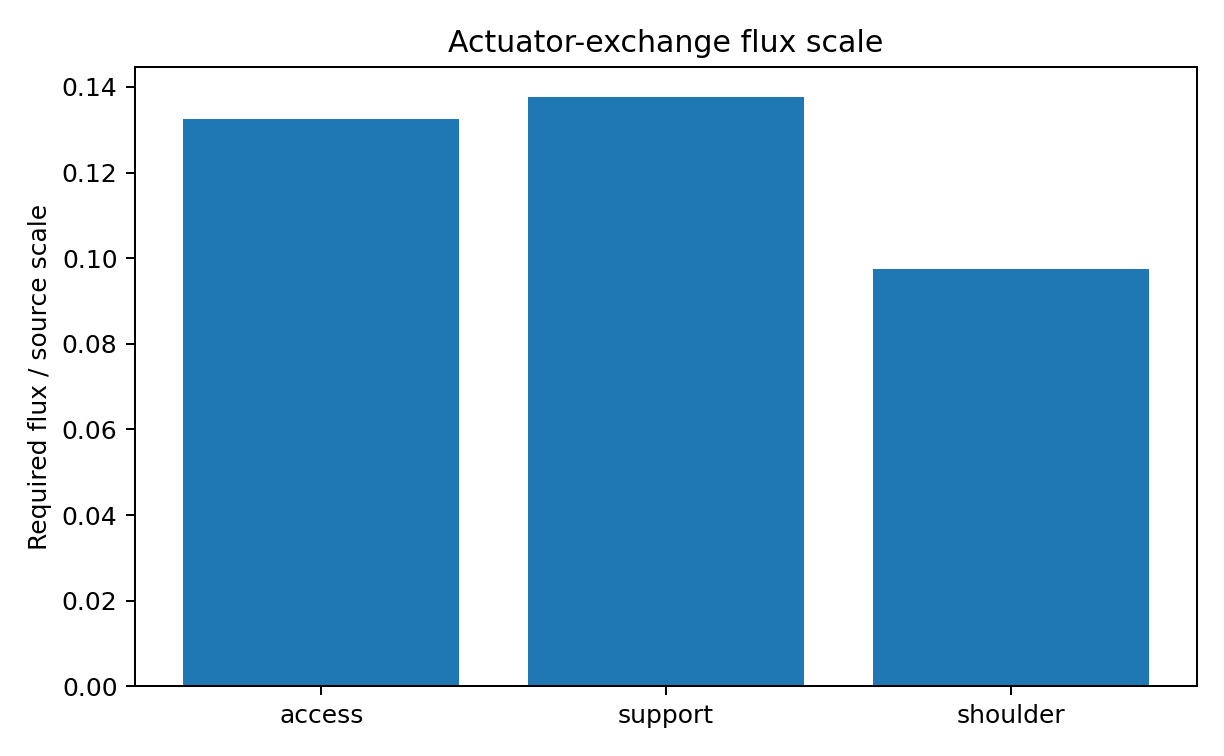
\includegraphics[width=0.72\linewidth]{../figures/actuator_exchange_flux_scale.png}
\caption{Actuator-exchange flux scale by zone.  The reduced closure keeps the flux-completing channel bounded relative to the source scale.}
\label{fig:flux_scale}
\end{figure}

\section{Full-cycle flux-completed ledgers}

The strict readout applies Eq.~\eqref{eq:flux_completed} to account for the unfavorable radial null direction.  The full-cycle positive-to-negative ratios are given in Table~\ref{tab:full_cycle_ratios}.

\begin{table}[ht]
\centering
\caption{Flux-completed full-cycle positive-to-negative ratios for the primary observer families.}
\label{tab:full_cycle_ratios}
\begin{tabular}{lr}
\toprule
Observer family & Flux-completed full-cycle ratio \\
\midrule
Core line & 1.083 \\
Access mean & 1.471 \\
Support mean & 2.801 \\
Support-ring mean & 1.135 \\
Shoulder mean & 1.130 \\
\bottomrule
\end{tabular}
\end{table}

\begin{figure}[ht]
\centering
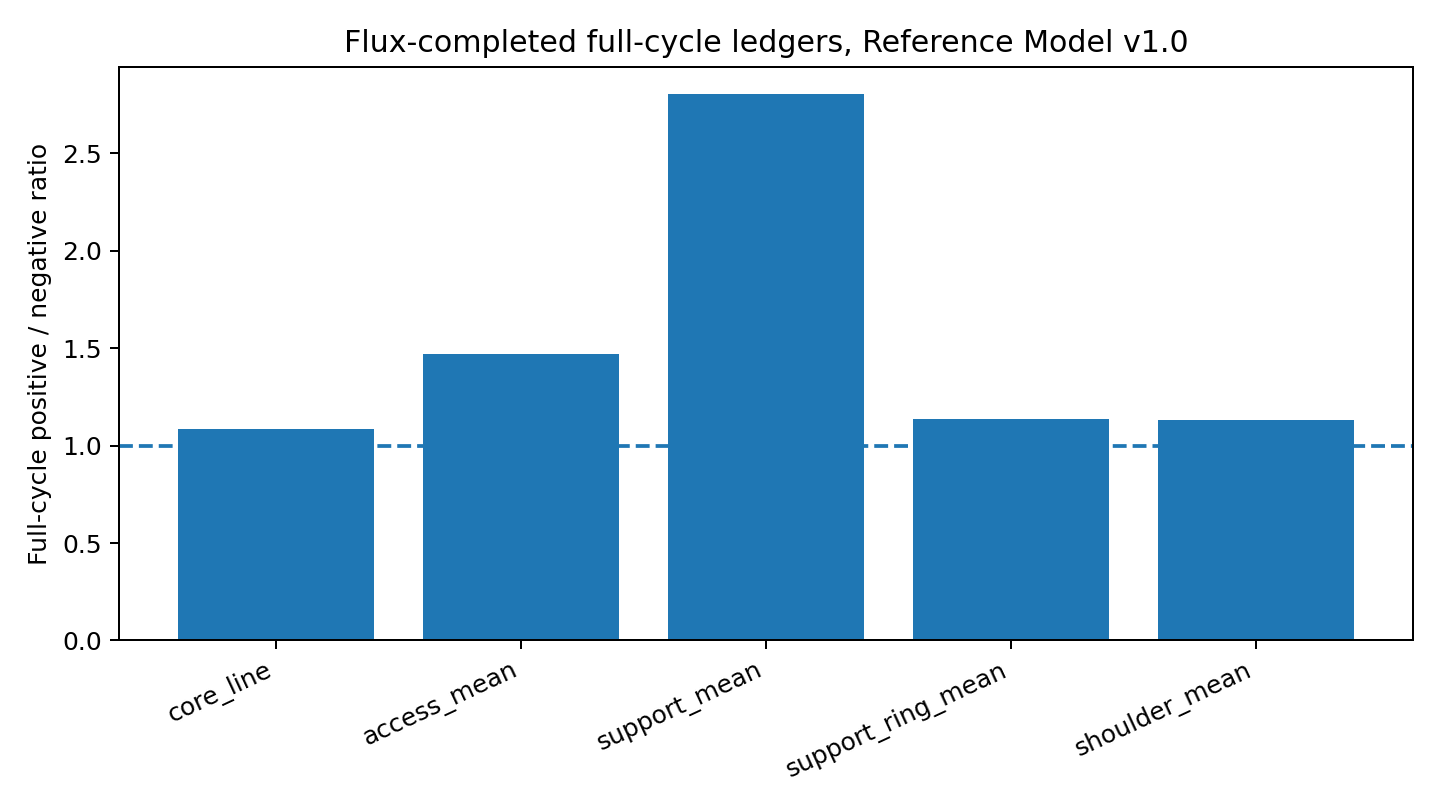
\includegraphics[width=0.72\linewidth]{../figures/flux_completed_full_cycle_ratios.png}
\caption{Flux-completed full-cycle ratios.  All primary observer-family ledgers clear unity in the reduced closure.}
\label{fig:ledger_ratios}
\end{figure}

These results are the engineering closure of the reduced model.  The source architecture, radial flux channel, and repayment phases produce closed ledgers for the core, access, support, support-ring, and shoulder families.

\section{Sampled-stress physics gate}

The active quantum-source gate is the Lorentzian sampled-stress proxy.  The screen uses
\begin{equation}
 \langle T_{kk}\rangle_\tau \gtrsim -\frac{C}{\tau^4},
 \qquad
 C=\frac{3}{32\pi^2}.
 \label{eq:qi_proxy}
\end{equation}
The flux-completed source has negative margins for the sampled windows listed in Table~\ref{tab:qi_margins}.  The table gives the most constraining window from the reduced screen for each observer family.

\begin{table}[ht]
\centering
\caption{Worst Lorentzian sampled-stress proxy margins for the flux-completed source.}
\label{tab:qi_margins}
\begin{tabular}{lrrr}
\toprule
Observer family & Worst margin & Window $\tau$ & Center \\
\midrule
Core line & $-1.062\times10^{-3}$ & 5.0 & 177.06 \\
Access mean & $-1.032\times10^{-3}$ & 5.0 & 177.06 \\
Support mean & $-8.215\times10^{-3}$ & 2.0 & 8.58 \\
Support-ring mean & $-2.746\times10^{-2}$ & 2.0 & 8.58 \\
Shoulder mean & $-8.607\times10^{-3}$ & 2.0 & 8.58 \\
\bottomrule
\end{tabular}
\end{table}

\begin{figure}[ht]
\centering
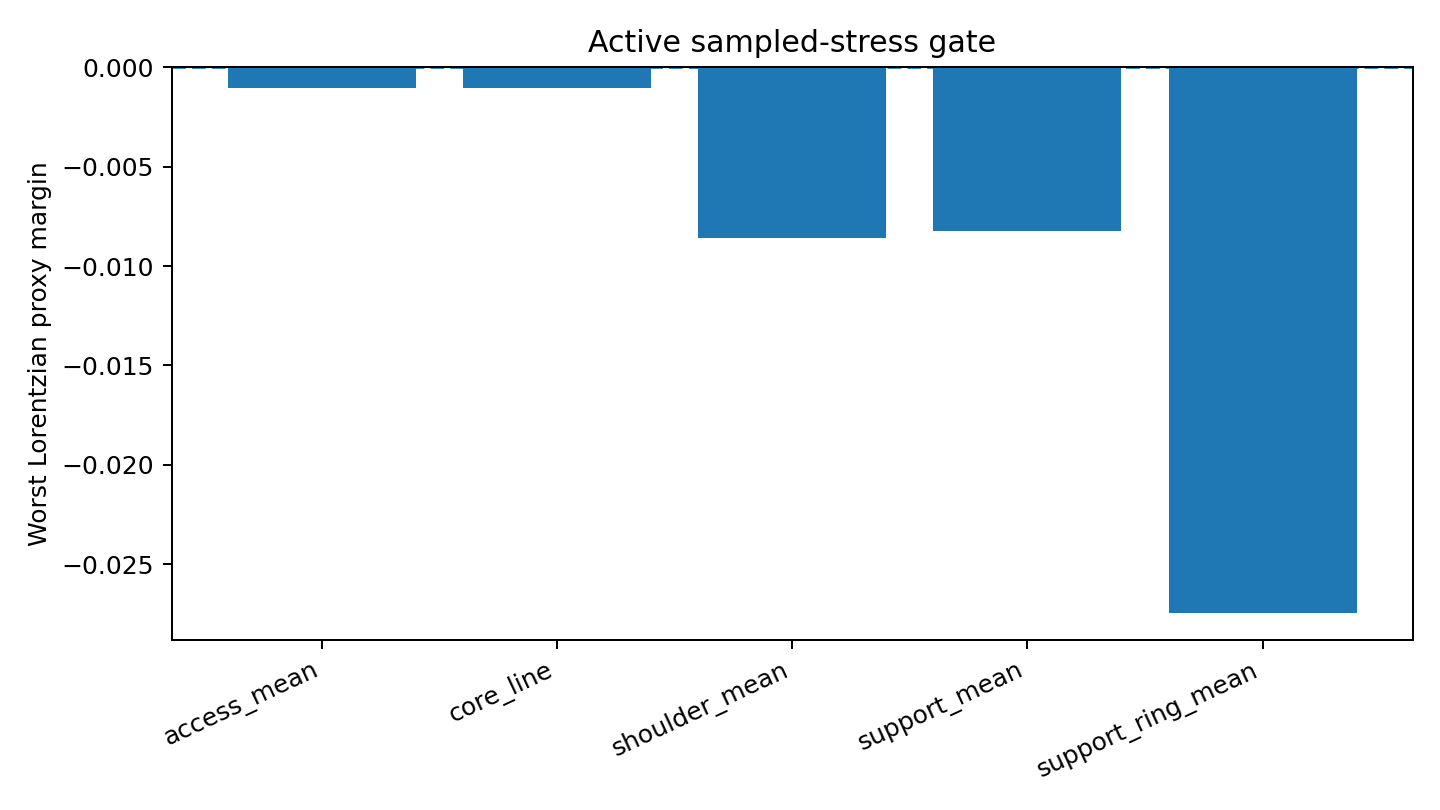
\includegraphics[width=0.72\linewidth]{../figures/worst_lorentzian_proxy_margins.png}
\caption{Worst Lorentzian proxy margins for the frozen reduced model.  The sampled-stress result supplies the active physics gate for the next source-admissibility phase.}
\label{fig:qi_margins}
\end{figure}

This screen gives the next target precisely.  The reduced engineering model closes geometry and ledgers, and the source-admissibility phase now evaluates the frozen source target against source-specific quantum inequalities, quantum-interest timing, NMC scalar field equations, and backreaction.

\section{Engineering interpretation}

The model supplies a complete reduced engineering architecture for the current phase.  The geometry control, observer ledgers, source roles, and closure check are connected by a single workflow:
\begin{equation}
 \hbox{geometry control}
 \rightarrow
 \hbox{observer-family ledger}
 \rightarrow
 \hbox{source role}
 \rightarrow
 \hbox{closure check}
 \rightarrow
 \hbox{physics gate}.
 \label{eq:workflow}
\end{equation}
The main design-level findings are:
\begin{enumerate}
\item $B(l,t)$ is a support-dilution actuator.  It reduces local support severity and prepares the radial infrastructure.
\item $R(l,t)$ is a flare/access-state actuator.  It opens the flared access state after prestretch and closes it before repayment.
\item $N(l,t)$ is a timing and matching actuator.  It shapes the shoulder and supports access isolation.
\item The source sector is best organized by roles.  The NMC-like component carries core/access support, while infrastructure and shoulder components carry repayment and matching.
\item Flux-completed anisotropic closure converts the source ledger into a reduced actuator-exchange tensor with bounded flux and small residual.
\item The Lorentzian sampled-stress screen supplies the active quantum-source gate and turns the remaining physics problem into a concrete target.
\end{enumerate}
This organization is the paper's scientific and engineering utility.  It makes the source problem reproducible and decomposed.

\section{Reproducibility package}

The accompanying bundle contains the LaTeX source, PDF, scripts, data tables, figures, literature access notes, and manifest.  The main scripts are:
\begingroup\small
\begin{itemize}
\item \path{run_invariant_packet_v03.py}: frozen-geometry invariant and observer-family diagnostics;
\item \path{run_source_realism_prescreen_v02.py}: phase-structured source ledger screen;
\item \path{run_candidate_source_model_v02.py}: full NMC scalar-channel compatibility screen;
\item \path{run_candidate_source_model_v03_component_polish.py}: component separation and locality polish;
\item \path{run_candidate_source_model_v03p1_residual_balance.py}: residual infrastructure-repayment balance;
\item \path{run_hybrid_source_closure_v01.py}: reduced anisotropic closure;
\item \path{run_hybrid_source_closure_v01p1_fluxmin_rebalance.py}: strict flux-completed rebalance.
\end{itemize}
\endgroup
The data folder includes the observer ledgers, closure summaries, sampled-stress tables, source-component scores, and extracted summaries used in the paper.

\section{Scope and next phase}

The frozen result is
\begin{equation}
 \boxed{\hbox{Hybrid Flare-Gated Reduced Reference Model v1.0}}.
\end{equation}
Its status is summarized in Table~\ref{tab:status}.

\begin{table}[ht]
\centering
\caption{Gate status for the reduced reference model.}
\label{tab:status}
\begin{tabular}{p{0.45\linewidth}p{0.4\linewidth}}
\toprule
Gate & Status \\
\midrule
Geometry lifecycle & Frozen as Reference Geometry v0.3 \\
Source architecture & Frozen as Hybrid Source Architecture v0.3 \\
Component separation & NMC support plus infrastructure repayment plus shoulder/matching \\
Flux-completed ledgers & Primary observer-family ratios above unity \\
Reduced conservation & Small residual with bounded actuator-exchange flux \\
Access isolation & Preserved in the reduced screens \\
Lorentzian sampled-stress proxy & Active quantum-source gate \\
Physical source construction & Next phase \\
Backreaction/stability & Next phase \\
\bottomrule
\end{tabular}
\end{table}

The next phase evaluates quantum-source admissibility for the frozen target.  The work items are: field-equation closure for the NMC-like support component, actuator-exchange interpretation for infrastructure repayment, source-specific quantum inequalities, quantum-interest timing for each negative/positive source pair, perturbative backreaction across flare opening and closure, and repeated-operation accumulation in the support-ring and shoulder components.

\section{Conclusion}

This paper constructs a phase-structured reduced reference model for wormhole-support infrastructure.  The model uses $B$ as a radial support-dilution actuator, $R$ as a flare/access-state actuator, $N$ as a timing and shoulder-matching actuator, and a hybrid source sector that separates NMC-like support from infrastructure repayment and shoulder/matching.  The final reduced closure embeds the source ledger in an anisotropic tensor with conservation-completing radial flux.  The flux-completed full-cycle ledgers close for the core, access, support, support-ring, and shoulder observer families, and the conservation residual remains small in the reduced embedding.

The model supplies a frozen target for the next physical gate.  Its Lorentzian sampled-stress screen identifies the active quantum-source admissibility problem with explicit observer families, sampling windows, and margins.  The result is therefore a reproducible engineering reference model and a concrete source-admissibility benchmark for future semiclassical, scalar-field, and backreaction studies.


\begin{thebibliography}{11}

\bibitem{morris_thorne_1988}
Michael S. Morris and Kip S. Thorne.
\newblock Wormholes in spacetime and their use for interstellar travel: A tool for teaching general relativity.
\newblock \emph{American Journal of Physics}, 56(5):395--412, 1988.
\newblock \doi{10.1119/1.15620}.

\bibitem{ford_roman_1996}
L. H. Ford and Thomas A. Roman.
\newblock Quantum field theory constrains traversable wormhole geometries.
\newblock \emph{Physical Review D}, 53:5496--5507, 1996.
\newblock \doi{10.1103/PhysRevD.53.5496}; arXiv:gr-qc/9510071.

\bibitem{ford_roman_1999}
L. H. Ford and Thomas A. Roman.
\newblock The quantum interest conjecture.
\newblock \emph{Physical Review D}, 60:104018, 1999.
\newblock \doi{10.1103/PhysRevD.60.104018}; arXiv:gr-qc/9901074.

\bibitem{visser_kar_dadhich_2003}
Matt Visser, Sayan Kar, and Naresh Dadhich.
\newblock Traversable wormholes with arbitrarily small energy condition violations.
\newblock \emph{Physical Review Letters}, 90:201102, 2003.
\newblock \doi{10.1103/PhysRevLett.90.201102}; arXiv:gr-qc/0301003.

\bibitem{kar_dadhich_visser_2004}
Sayan Kar, Naresh Dadhich, and Matt Visser.
\newblock Quantifying energy condition violations in traversable wormholes.
\newblock \emph{Pramana}, 63:859--864, 2004.
\newblock \doi{10.1007/BF02705207}; arXiv:gr-qc/0405103.

\bibitem{fewster_roman_2005}
Christopher J. Fewster and Thomas A. Roman.
\newblock On wormholes with arbitrarily small quantities of exotic matter.
\newblock \emph{Physical Review D}, 72:044023, 2005.
\newblock \doi{10.1103/PhysRevD.72.044023}; arXiv:gr-qc/0507013.

\bibitem{hochberg_visser_1998}
David Hochberg and Matt Visser.
\newblock The null energy condition in dynamic wormholes.
\newblock \emph{Physical Review Letters}, 81:746--749, 1998.
\newblock \doi{10.1103/PhysRevLett.81.746}; arXiv:gr-qc/9802048.

\bibitem{kuhfittig_2002}
Peter K. F. Kuhfittig.
\newblock Static and dynamic traversable wormhole geometries satisfying the Ford--Roman constraints.
\newblock \emph{Physical Review D}, 66:024015, 2002.
\newblock \doi{10.1103/PhysRevD.66.024015}.

\bibitem{barcelo_visser_2000}
Carlos Barcel\'{o} and Matt Visser.
\newblock Scalar fields, energy conditions, and traversable wormholes.
\newblock \emph{Classical and Quantum Gravity}, 17:3843--3864, 2000.
\newblock \doi{10.1088/0264-9381/17/18/318}; arXiv:gr-qc/0003025.

\bibitem{gao_jafferis_wall_2017}
Ping Gao, Daniel Louis Jafferis, and Aron C. Wall.
\newblock Traversable wormholes via a double trace deformation.
\newblock \emph{Journal of High Energy Physics}, 2017:151, 2017.
\newblock \doi{10.1007/JHEP12(2017)151}; arXiv:1608.05687.

\bibitem{bobrick_martire_2021}
Alexey Bobrick and Gianni Martire.
\newblock Introducing physical warp drives.
\newblock \emph{Classical and Quantum Gravity}, 38:105009, 2021.
\newblock \doi{10.1088/1361-6382/abdf6e}; arXiv:2102.06824.

\end{thebibliography}


\end{document}
